\chapter{Finding faces}
OpenIMAJ contains a set of classes that contain implementations of some of the state-of-the-art face 
detection and recognition algorithms. These classes are provided as a sub-project of the OpenIMAJ 
code-base called \verb+faces+. The OpenIMAJ maven archetype adds the face library as a dependency and 
so we can start building face detection applications straight away.

Create a new application using the quick-start archetype (see tutorial 1) and import it into your IDE. 
If you look at the \verb+pom.xml+ file you will see that the \verb+faces+ dependency from OpenIMAJ is 
already included. As you've already done the video-processing tutorial, we'll try to find faces within 
the video that your webcam produces. If you don't have a webcam, follow the video tutorial on how to 
use video from a file instead.

Start by removing the code from the main method of the \verb+App.java+ class file. Then create a video 
capture object and a display to show the video. Create a listener on the video display to which we can 
hook our face finder. The code is below, but check out the previous tutorial on video processing if 
you're not sure what it means.
\begin{lstlisting}[language=java]
VideoCapture vc = new VideoCapture( 320, 240 );
VideoDisplay<MBFImage> vd = VideoDisplay.createVideoDisplay( vc );
vd.addVideoListener( 
  new VideoDisplayListener<MBFImage>() {
    @Override
    public void beforeUpdate( MBFImage frame ) {
    }

    @Override
    public void afterUpdate( VideoDisplay<MBFImage> display ) {
    }
  });
\end{lstlisting}
For finding faces in images (or in this case video frames) we use a face detector. The \verb+FaceDetector+ 
interface provides the API for face detectors and there are currently two implementations within OpenIMAJ - 
the \verb+HaarCascadeDetector+ and the \verb+SandeepFaceDetector+. The \verb+HaarCascadeDetector+
is considerably more robust than the \verb+SandeepFaceDetector+, so we'll use that.

In the \verb+beforeUpdate()+ method, instantiate a new \verb+HaarCascadeDetector+. The constructor takes 
the minimum size in pixels that a face can be detected at. For now, set this to \verb+40+ pixels:
\begin{lstlisting}[language=java]
FaceDetector<DetectedFace,FImage> fd = new HaarCascadeDetector(40);
\end{lstlisting}

Like all \verb+FaceDetector+ implementations, the \verb+HaarCascadeDetector+ has a method \verb+detectFaces()+
which takes an image. Because the \verb+HaarCascadeDetector+ uses single band images, we must convert 
our multi-band colour image into a single band image. To do this we can use the \verb+Transforms+ utility 
class that contains some static methods for converting images. The \verb+calculateIntensity()+ method 
will do just fine. Note that functionally the \verb+calculateIntensity()+ method does the same thing 
as the \verb+flatten()+ method we used earlier when used on RGB images.
\begin{lstlisting}[language=java]
List<DetectedFace> faces = fd.detectFaces(Transforms.calculateIntensity(frame));
\end{lstlisting}
The \verb+detectFaces()+ method returns a list of \verb+DetectedFace+ objects which contain 
information about the faces in the image. From these objects we can get the rectangular 
bounding boxes of each face and draw them back into our video frame. As we're doing all 
this in our \verb+beforeUpdate()+ method, the video display will end up showing the 
bounding boxes on the displayed video. If you run the code and you have a webcam attached,
you should see yourself with a box drawn around your face. The complete code is shown below:
\begin{lstlisting}[language=java]
FaceDetector<DetectedFace,FImage> fd = new HaarCascadeDetector(40);
List<DetectedFace> faces =
            fd.detectFaces( Transforms.calculateIntensity(frame));

for( DetectedFace face : faces ) {
    frame.drawShape(face.getBounds(), RGBColour.RED);
}
\end{lstlisting}
\marginpar{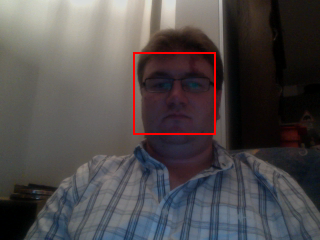
\includegraphics[width=\marginparwidth]{face-bounds.png}}
OpenIMAJ has other face detectors which go a bit further than just finding the face. 
The \verb+FKEFaceDetector+ finds facial keypoints (the corners of the eyes, nose and mouth) 
and we can use this detector instead simply by instantiating that object instead of the 
\verb+HaarCascadeDetector+. The \verb+FKEFaceDetector+ returns a slightly different object 
for each detected face, called a \verb+KEDetectedFace+. The \verb+KEDetectedFace+ object 
contains the extra information about where the keypoints in the face are located. 
The lines of our code to instantiate the detector and detect faces can now be changed to 
the following:
\begin{lstlisting}[language=java]
FaceDetector<KEDetectedFace,FImage> fd = new FKEFaceDetector();
List<KEDetectedFace> faces = fd.detectFaces( Transforms.calculateIntensity( frame ) );
\end{lstlisting}
If you run the demo now, you will see exactly the sameas before, as the \verb+FKEFaceDetector+ 
still detects bounding boxes. It may be running a bit slower though, as there is much more 
processing going on - we're just not seeing the output of it! So, let's plot the facial keypoints.

To get the keypoints use \verb+getKeypoints()+ on the detected face. Each keypoint has a 
position (public field) which is relative to the face, so we'll need to translate the 
point to the position of the face within the video frame before we plot the points. 
To do that we can use the \verb+translate()+ method of the \verb+Point2d+ class
and the \verb+minX()+ and \verb+minY()+ methods of the \verb+Rectangle+ class.

\section*{Exercises}
\subsection*{Exercise 1: Drawing facial keypoints}
Use the information above to plot the facial keypoints on the video.
\marginpar{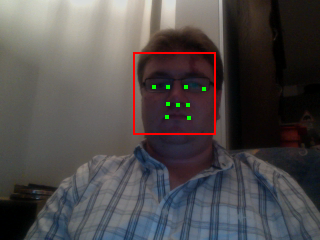
\includegraphics[width=\marginparwidth]{face-points.png}}

\subsection*{Exercise 2: Speech bubbles}
Try and take the speech bubble from the previous image tutorial and make it come from the mouth 
in the video. \textbf{Hints:} use \verb+getKeypoint(FacialKeypointType)+ to get the keypoint 
of the left corner of the mouth and plot the ellipses depending on that point. You may need to 
use smaller ellipses and text if your video is running at 320x240.
\marginpar{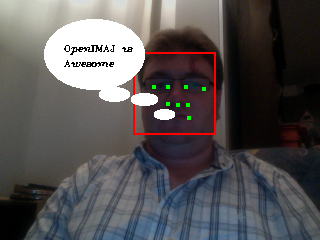
\includegraphics[width=\marginparwidth]{face-awesome.png}}
